\subsection{Prefazione}
 \begin{frame} {Metodologia Applicata}
  Per lo sviluppo del processo software descritto a breve, è stata applicata la metodologia dell'Unifiled Process (UP) suggerita
  durante il corso di studi di Ingegneria del Software.
   \begin{figure}
     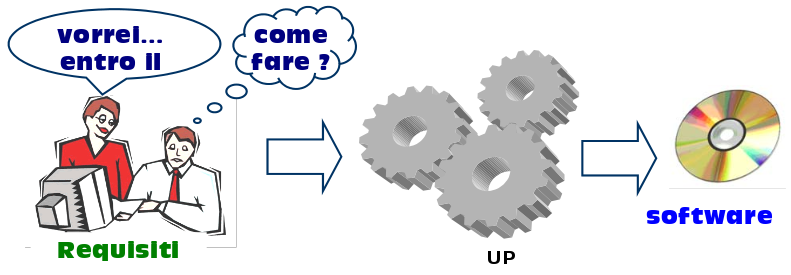
\includegraphics[scale=0.40]{image/Up_sep.png}{\centering}
    \caption{Software Engineering Process} 
    \label{fig_SEP}
   \end{figure}
 \end{frame}

 \begin{frame} {Struttura di UP}
    Il ciclo di vita del progetto è diviso in quattro fasi: Ideazione (Inception), Elaborazione (Elaboration), Costruzione (Construction)
    e Transizione (Transition), come si può vedere nella figura \ref{fig_US}. 
   \begin{figure}
     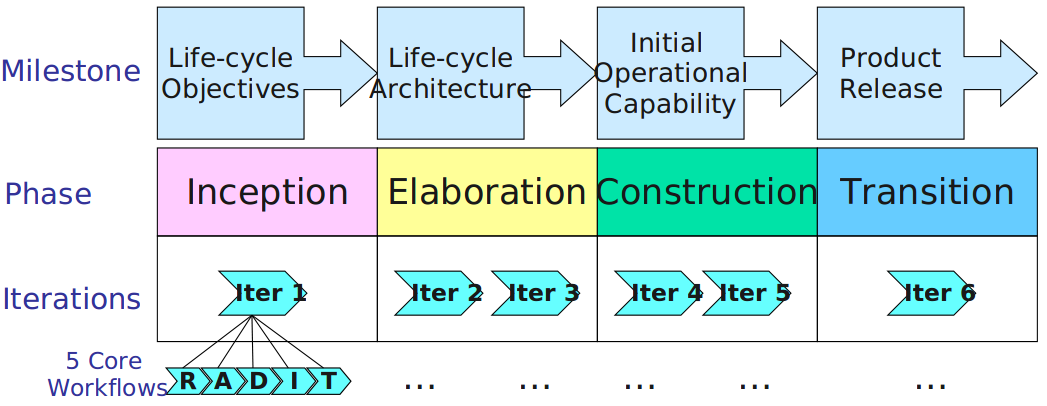
\includegraphics[scale=0.26]{image/Up_Structure.png}{\centering}
    \caption{Fasi dell'Unified Process} 
    \label{fig_US}
   \end{figure}
  \end{frame}

 \begin{frame} {Struttura di UP}
   Ogni fase è formata da una o più iterazioni. Per ogni iterazione si sviluppano in modo iterativo e incrementale 5 attività di lavoro 
   (workflows) RADIT: Requisiti (Requirements), Analisi (Analsys), Progettazione (Design), Implementazione (Implementation)e Test, come si 
   può vedere nella figura \ref{fig_UIW}.
   \begin{figure}
     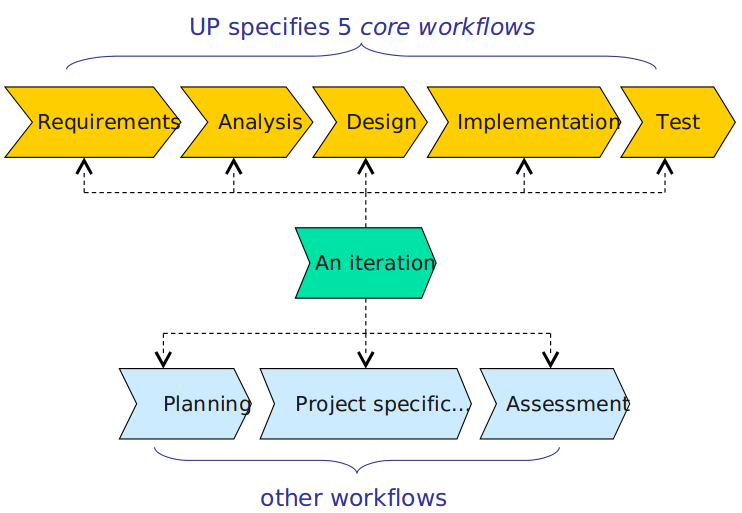
\includegraphics[scale=0.20]{image/Up_Iteration_Workflows.png}{\centering}
    \caption{Iterazioni dell'Unifiled Process} 
    \label{fig_UIW}
   \end{figure}
  \end{frame}

 \begin{frame} [allowframebreaks] {Documenti del progetto realizzati }
   Gli elementi che costituiscono il progetto realizzato sono:
   \begin{enumerate} 
     \item Documento di Visione;
     \item Glossario;
     \item Diagrammi dei casi d'uso;
     \item Descrizione dei casi d'uso in formato breve e dettagliato;
     \item Prototipo UI (User Interface);
     \item Modelli di dominio del sistema dei vari casi d'uso in formato dettagliato;
     \item Diagrammi - Oggetti di dominio del sistema dei vari casi d'uso in formato dettagliato;
     \item Diagrammi - Sequenza di dominio dei vari casi d'uso in formato dettagliato ;
     \item Contratti delle operazioni;
     \item System Sequence Diagram (SSD) e Domain Class Diagrams (DCD) di progetto del sistema dei vari casi d'uso in formato dettagliato;
     \item Codice sorgente dei diagrammi UML realizzati con Astah;
     \item Software del progetto che comprende i casi d'uso in fomato dettagliato scritto in linguaggio a oggetti Java, 
           con l'utilizzo di NetBeans IDE 8.0;
     \item Test del software realizzati tramite JUnit 4.0; 
     \item Documentazione tramite la Javadocs del codice sorgente; 
     \item Guida utente dell'avvio e configurazione del software realizzato;
     \item Documenti di installazione, downloading dei repository di GitHub;
     \item Documentazione realizzata in \LaTeX.
   \end{enumerate}
 \end{frame}
